\chapter{基于变量消除的精确推断}
\label{chap:pgm-elimination}

设备报警后，诊断任务可以有两种输出：给出故障的后验概率，或选出一组最可能的故障、过热和传感器状态。两种输出使用同一组局部因子，却以不同方式汇总未知状态。本章从第~\ref{sec:pgm-representations-local-computation}节的因子组合与消元操作出发，给出完整算法及其正确性证明。对$d$个二元变量，直接枚举需访问$2^d$个配置；利用局部分解减少重复计算，是精确推断的主要任务。

查询通常只保留部分变量，其余变量的影响可以汇总成剩余变量上的函数，供后续步骤使用。\term{变量消除}（variable elimination, VE）据此逐个收集含有当前变量的因子，将它们相乘，再以求和、积分或最大化消去该变量；所得新因子替换桶内函数，保存它们对剩余变量的共同影响。本章分别说明替换为何保留查询答案、查询为何选择不同算子，以及顺序怎样改变中间作用域。离散因子以状态组合数表示规模，高斯因子则以矩阵块维度表示规模，两种表示由此产生不同的计算代价。

\section{推断问题与因子运算}
\label{sec:pgm-elimination-factor-operations}

\subsection{查询、证据与消元变量}
\label{sec:pgm-elimination-query-evidence}

求故障后验时，要固定报警证据，保留故障变量，并汇总其余未知状态。一般地，模型的节点集合为$V$，节点$i$对应随机变量$X_i$；已观测节点组成$O\subseteq V$，取值为$\bm{x}_O=\bm{e}$，查询节点组成$Q\subseteq V\setminus O$。待消元节点为$R=V\setminus(O\cup Q)$。三个大写集合指定变量角色，$\bm{x}_Q$才是一组查询状态。证据集合用$O$记，以便与图的边集合$E$区分。

以下把模型参数视为已知输入。设共有$m$个非负因子$\psi_a$，其完整乘积具有有限且非零的归一化常数$Z$，联合分布写为
\begin{equation}
  p(\bm{x})=\frac{1}{Z}\prod_{a=1}^{m}\psi_a(\bm{x}_{S_a}),
  \qquad S_a\subseteq V.
  \label{eq:pgm-elimination-factorization}
\end{equation}
有向模型采用局部条件概率作为因子，完整积已归一化，故$Z=1$。无向模型的势需由全局$Z$归一化。这些函数都是当前推断的输入，第~\ref{chap:pgm-parameter-learning}章再讨论如何从数据估计它们。

把证据坐标固定在观测值后，原乘积成为未观测变量上的函数：
\begin{equation}
  F_{\bm{e}}(\bm{x}_{V\setminus O})
  =\left.\prod_{a=1}^{m}\psi_a(\bm{x}_{S_a})
  \right|_{\bm{x}_O=\bm{e}}.
  \label{eq:pgm-elimination-evidence-function}
\end{equation}
先取各变量状态数有限的离散情形。汇总$R$的联合状态得到查询权重，再对$Q$的所有状态归一化：
\begin{equation}
  \begin{aligned}
    g_Q(\bm{x}_Q)
      &=\sum_{\bm{x}_R}F_{\bm{e}}(\bm{x}_Q,\bm{x}_R),\\
    Z_{\bm{e}}&=\sum_{\bm{x}_Q}g_Q(\bm{x}_Q),\\
    p(\bm{x}_Q\mid\bm{e})&=\frac{g_Q(\bm{x}_Q)}{Z_{\bm{e}}}.
  \end{aligned}
  \label{eq:pgm-elimination-marginal-query}
\end{equation}
下标$\bm{x}_R$遍历待消元变量的联合状态。总权重满足$Z_{\bm{e}}=Zp(\bm{e})$，因此计算条件概率时原$Z$在分子分母中抵消，可以直接从因子积开始。后验比值在$Z_{\bm{e}}>0$的证据事件上有定义；模型赋予观测零概率时，该比值的分母为零。

连续变量用积分汇总未知坐标。联合密度存在且积分有限时，式~\eqref{eq:pgm-elimination-marginal-query}的积分版本给出边缘条件密度。连续观测处的$p(\bm{e})$表示边缘密度值，比值只在密度有限且为正的观测处使用。形式相同的查询还需配合适当的函数表示，才能解析完成积分。

\subsection{因子乘积}
\label{sec:pgm-elimination-factor-product}

相乘两张因子表时，需要按变量身份及状态含义对齐坐标。\term{作用域}（scope）指定因子的自变量，也指定消元后需要保留的坐标。若$D_i$是$X_i$的取值集合，作用域为$S$的离散因子是非负函数$\psi_S:\prod_{i\in S}D_i\to[0,\infty)$。存储表时还要记下$S$内变量的排列和状态编码：同一变量可以位于不同表轴上，但相乘时同一个状态必须有相同含义。

两个函数分别使用$A$与$B$中的变量，乘积便使用它们的并集$A\cup B$：
\begin{equation}
  (\psi_A\psi_B)(\bm{x}_{A\cup B})
  =\psi_A(\bm{x}_A)\psi_B(\bm{x}_B).
  \label{eq:pgm-elimination-product}
\end{equation}
对$A\cup B$的一组取值，两因子各读取自己的坐标，其中共享变量取同一状态。例如，$\psi_{\{F,H\}}(f,h)\psi_{\{H,S\}}(h,s)$以$(f,h,s)$为索引；计算$(0,1,0)$时，分别读取前表$(0,1)$与后表$(1,0)$。三个变量均为二元时，两张$4$项表的乘积共有$8$项，新增的坐标来自两表作用域的并集。

因子保存相对权重，其全表求和可以异于$1$。空作用域的因子是标量，也参与完整乘积；条件概率比较中的公共尺度可约去，而证据概率或绝对得分需要这些尺度。乘积还要保留函数的出现次数：两个数值相同的因子仍相乘两次。以下的$\mathcal{F}$因此按多重集合使用。

\subsection{因子约简与边缘化}
\label{sec:pgm-elimination-reduction-marginalization}

观测把一个变量的状态固定后，可以从因子表读取相应切片。把证据代入并从作用域移去固定坐标，称为\term{因子约简}（factor reduction）。报警证据$A=1$将$p(a\mid h,s)$变为$\ell_A(h,s)=p(A=1\mid h,s)$，表示各$(h,s)$状态对该报警的支持权重。结合先验与其他因子、再统一归一化，才能得到这些原因的后验分布。

对状态仍未知的变量，概率查询要汇总其全部取值。\term{边缘化}（marginalization）把这些权重相加，留下其余坐标上的函数：若$i\in S$，则
\begin{equation}
  (\mathop{\textstyle\sum}_{x_i}\psi_S)
    (\bm{x}_{S\setminus\{i\}})
  =\sum_{x_i\in D_i}\psi_S(\bm{x}_{S\setminus\{i\}},x_i).
  \label{eq:pgm-elimination-factor-marginal}
\end{equation}
约简读取已知状态下的切片，边缘化累加未知状态。两种操作都减少自变量数，分别保留观测条件下的权重与未知变量的总贡献。

一个未知变量可能同时影响多个因子，汇总时需要让它们共享同一个状态。若$X_i$出现在$\psi_1(x_i,y)$和$\psi_2(x_i,z)$中，正确的新因子为$\sum_{x_i}\psi_1(x_i,y)\psi_2(x_i,z)$。分别求和后相乘，会允许两张表使用不同的$x_i$，改变原函数的共享坐标约束。因此，消元先收集所有含$X_i$的因子，再对共同乘积汇总；新函数保留它们在剩余坐标上的联合影响。

完成非查询变量的边缘化后，查询权重可以统一归一化。中途若用一个与全部自变量无关的正常数缩放因子，最终条件概率的公共尺度仍会抵消，但计算$Z_{\bm{e}}$需记录并补回该常数。逐行归一化的除数随剩余坐标变化，会改变各查询配置的相对权重，因而属于对函数的实质修改。

\section{边缘概率的变量消除算法}
\label{sec:pgm-elimination-sum-product}

\subsection{从朴素枚举到分配律}
\label{sec:pgm-elimination-distributivity}

沿用报警模型作为可逐项计算的例子：故障$F$、过热$H$、报警$A$和传感器失灵$S$均取$0$或$1$。联合分解为
\begin{equation}
  p(f,h,a,s)=p(f)p(h\mid f)p(s)p(a\mid h,s).
  \label{eq:pgm-elimination-alarm-model}
\end{equation}
有向结构$F\to H\to A\leftarrow S$使两个根节点$F,S$独立。设置$p(F=1)=0.1$、$p(S=1)=0.05$，并取
\[
  p(H=1\mid F=0)=0.1,\qquad
  p(H=1\mid F=1)=0.8.
\]
表~\ref{tab:pgm-elimination-alarm-cpt}给出四种$(h,s)$下的报警概率；二元分布的状态$0$概率都由$1$减去状态$1$概率得到。这组人工参数只用于解释消元步骤。

\begin{table}[htbp]
  \centering
  \begin{tabular}{ccc}
    \toprule
    $h$ & $s$ & $p(A=1\mid h,s)$\\
    \midrule
    $0$ & $0$ & $0.01$\\
    $1$ & $0$ & $0.90$\\
    $0$ & $1$ & $0.70$\\
    $1$ & $1$ & $0.99$\\
    \bottomrule
  \end{tabular}
  \caption{报警模型的人工条件表。每行固定$(h,s)$并列出$p(A=1\mid h,s)$，同一行的不报警概率为$1-p(A=1\mid h,s)$。}
  \label{tab:pgm-elimination-alarm-cpt}
\end{table}

将$A=1$代入报警因子后，故障查询需要累加过热和传感器的全部状态：
\[
  g_F(f)=\sum_h\sum_s p(f)p(h\mid f)p(s)\ell_A(h,s).
\]
直接枚举对每个$f$访问全部$(h,s)$，共需访问$8$个三元配置。其中$p(s)\ell_A(h,s)$不使用$f$，可以让两种故障状态共享这部分结果。利用乘法对加法的分配律，先对$s$汇总与它相关的两个函数：
\begin{equation}
  g_F(f)
  =p(f)\sum_h p(h\mid f)
    \underbrace{\sum_s p(s)\ell_A(h,s)}_{\tau_S(h)}.
  \label{eq:pgm-elimination-alarm-reorder}
\end{equation}
所得$\tau_S(h)$替换$p(s)$与$\ell_A(h,s)$，对每种$h$计算一次，供所有$f$使用。下一步将$p(h\mid f)\tau_S(h)$对$h$求和，生成$f$上的函数。图~\ref{fig:pgm-elimination-alarm-buckets}将每步输入与输出的坐标分别画出。

\begin{figure}[htbp]
  \centering
  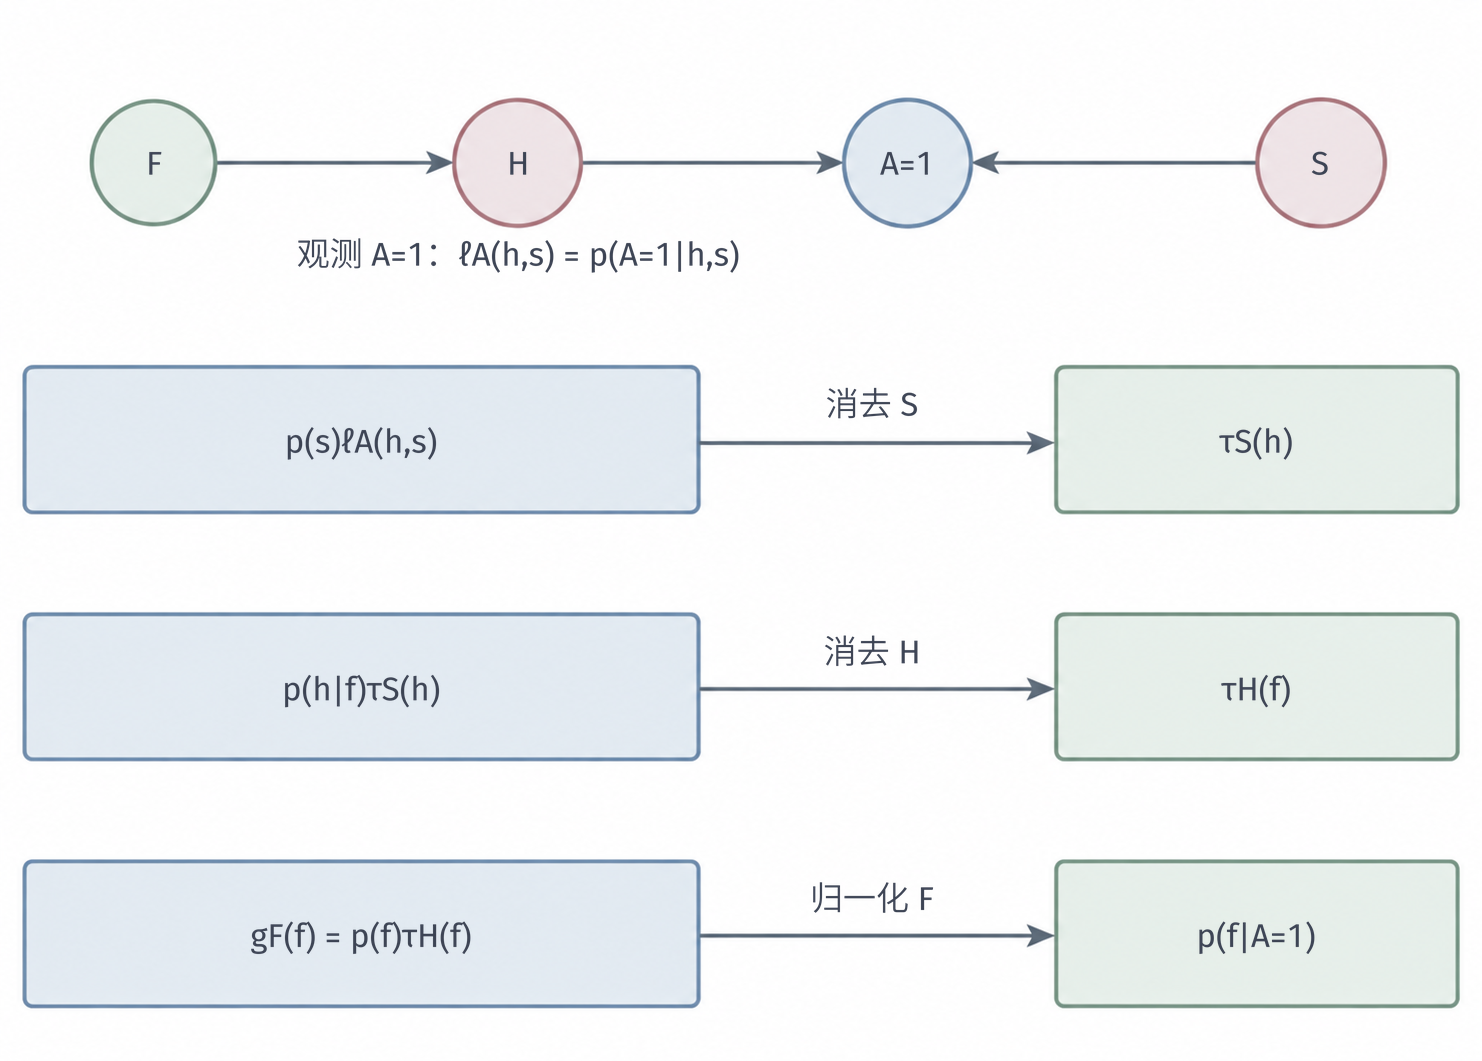
\includegraphics[width=112.000mm]{figures/06-probabilistic-graphical-models/02-inference/generated/pgm-elimination-alarm-buckets/figure.png}
  \caption{故障后验查询的两步消元。上方有向图以蓝色$A=1$标出证据；下方先从$p(s)\ell_A(h,s)$求和得到$\tau_S(h)$，再从$p(h\mid f)\tau_S(h)$求和得到$\tau_H(f)$。每步输出只保留尚未消去的坐标，$F$最终结合$p(f)$并归一化。}
  \label{fig:pgm-elimination-alarm-buckets}
\end{figure}

这种重排让后续故障状态复用同一局部汇总，每个$s,h$状态仍以原权重参与求和，所以代数结果与完整枚举相同。节省多少取决于输出函数的作用域：若一桶包含几乎全部剩余变量，形成的新表仍可能过大。选择顺序的目的，就是控制这类中间函数的坐标数和状态组合数。

\subsection{变量消除算法}
\label{sec:pgm-elimination-ve-algorithm}

一般因子分解也按同一方式替换局部乘积。证据约简后的初始因子多重集合记为$\mathcal{F}^{(0)}$，顺序$\pi=(i_1,\ldots,i_k)$将待消元集合$R$的每个节点列出恰好一次。第$t$步收集全部含$X_{i_t}$的因子：
\[
  \mathcal{B}_t
  =\{\psi\in\mathcal{F}^{(t-1)}:
      i_t\in\operatorname{scope}(\psi)\}.
\]
$\operatorname{scope}(\psi)$给出函数的作用域。当前收集的多重集合称为变量的\term{桶}（bucket），其中的函数需要共同参与本步求和。令$U_t$为它们作用域的并集，去掉当前变量后的集合为$N_t=U_t\setminus\{i_t\}$，局部更新写为
\begin{equation}
  \begin{aligned}
    \phi_t(\bm{x}_{U_t})&=\prod_{\psi\in\mathcal{B}_t}\psi,\\
    \tau_t(\bm{x}_{N_t})&=\sum_{x_{i_t}}\phi_t(\bm{x}_{U_t}).
  \end{aligned}
  \label{eq:pgm-elimination-local-sum}
\end{equation}
计算$\phi_t$时，先按式~\eqref{eq:pgm-elimination-product}对齐每个函数的坐标。桶外函数不含$X_{i_t}$，从本步求和提出后仍留在当前集合中。

\begin{algorithm}[离散边缘概率的变量消除]
  \label{alg:pgm-elimination-marginal}
  \begin{algorithmic}[1]
    \Require 非负有限因子$\{\psi_a\}$，证据$\bm{x}_O=\bm{e}$，查询集$Q$
    \Require $R=V\setminus(O\cup Q)$的排列$\pi=(i_1,\ldots,i_k)$
    \Ensure 查询因子$g_Q$及$Z_{\bm{e}}>0$时的条件分布
    \State 将证据代入各因子，得到$\mathcal{F}^{(0)}$；保留标量因子
    \State 对未出现在任何作用域中的未观测变量，加入其恒为$1$的一元因子
    \For{$t=1,\ldots,k$}
      \State 收集$\mathcal{B}_t$，令$U_t$为其作用域的并集
      \State 对齐坐标并求乘积$\phi_t=\prod_{\psi\in\mathcal{B}_t}\psi$
      \State 对$x_{i_t}$求和，得到$\tau_t(\bm{x}_{U_t\setminus\{i_t\}})$
      \State $\mathcal{F}^{(t)}\gets
        (\mathcal{F}^{(t-1)}\setminus\mathcal{B}_t)\cup\{\tau_t\}$
    \EndFor
    \State 在查询取值空间上计算$g_Q=\prod_{\psi\in\mathcal{F}^{(k)}}\psi$
    \State 计算$Z_{\bm{e}}=\sum_{\bm{x}_Q}g_Q(\bm{x}_Q)$
    \If{$Z_{\bm{e}}=0$}
      \State 返回证据与模型不相容，条件分布未定义
    \Else
      \State 返回$g_Q$、$Z_{\bm{e}}$及$g_Q/Z_{\bm{e}}$
    \EndIf
  \end{algorithmic}
\end{algorithm}

算法~\ref{alg:pgm-elimination-marginal}按出现次数移除桶内函数并加入新因子。若某个未观测变量未进入任何函数，加入恒为$1$的一元因子后，它的求和仍贡献状态数。$R=\varnothing$时没有消元步骤，$Q=\varnothing$时最终乘积是证据权重标量$Z_{\bm{e}}$。边缘查询输出汇总后的函数，各个已消变量的状态都参与了累加，因此输出无需配置回溯。

报警查询从$p(f)$、$p(h\mid f)$、$p(s)$和$\ell_A(h,s)$四因子开始。$S$桶由$p(s)$与$\ell_A(h,s)$组成，两种$h$下的新函数值分别为
\begin{equation}
  \begin{aligned}
    \tau_S(0)&=0.95\times0.01+0.05\times0.70=0.0445,\\
    \tau_S(1)&=0.95\times0.90+0.05\times0.99=0.9045.
  \end{aligned}
  \label{eq:pgm-elimination-alarm-s}
\end{equation}
用$\tau_S(h)$替换$S$桶后，当前集合为$\{p(f),p(h\mid f),\tau_S(h)\}$。接着将含$H$的两个函数相乘并求和，得到
\begin{equation}
  \begin{aligned}
    \tau_H(0)&=0.9\times0.0445+0.1\times0.9045=0.1305,\\
    \tau_H(1)&=0.2\times0.0445+0.8\times0.9045=0.7325.
  \end{aligned}
  \label{eq:pgm-elimination-alarm-h}
\end{equation}
余下$p(f)$与$\tau_H(f)$相乘，给出$g_F(0)=0.11745$、$g_F(1)=0.07325$，总权重为$0.19070$。原有向联合积的$Z=1$，因此此值也是证据概率$p(A=1)$。把故障状态$1$的权重除以总权重，得到
\begin{equation}
  p(F=1\mid A=1)
  =\frac{0.07325}{0.19070}
  \approx0.384111.
  \label{eq:pgm-elimination-alarm-posterior}
\end{equation}
报警使故障概率从$0.1$升至约$0.384$。无故障过热、传感器失灵以及小概率误报也能解释报警，它们的概率都进入求和分母；保留这些解释使后验仍低于$1$。

这个顺序只产生$\tau_S(h)$、$\tau_H(f)$两张一元表。变量较多的模型可先按消元顺序分桶：将输入因子交给作用域中最早待消的变量，每步新函数再交给后续相应桶。这种收集、合并、汇总的组织方式对应Dechter的桶消除算法\scite{pgm-elimination-dechter1999}

\subsection{多变量查询}
\label{sec:pgm-elimination-multivariate-query}

联合查询故障与传感器状态时，保留$Q=\{F,S\}$，仅消去$H$。所需结果使用$(f,s)$共同索引：
\begin{equation}
  g_{F,S}(f,s)
  =p(f)p(s)\sum_h p(h\mid f)\ell_A(h,s).
  \label{eq:pgm-elimination-joint-query}
\end{equation}
以$f=s=0$为例，先汇总两种过热状态，得到
\[
  \begin{aligned}
    g_{F,S}(0,0)
    &=0.9\times0.95\times(0.9\times0.01+0.1\times0.90)\\
    &=0.084645.
  \end{aligned}
\]
对其余三种$(f,s)$执行相同求和，即得到表~\ref{tab:pgm-elimination-joint-query}。

\begin{table}[htbp]
  \centering
  \begin{tabular}{ccc}
    \toprule
    $f$ & $g_{F,S}(f,0)$ & $g_{F,S}(f,1)$\\
    \midrule
    $0$ & $0.084645$ & $0.032805$\\
    $1$ & $0.068590$ & $0.004660$\\
    \bottomrule
  \end{tabular}
  \caption{报警证据下的未归一化$(F,S)$联合权重。四项共用归一化常数$0.19070$，得到$p(f,s\mid A=1)$；若各行分别归一化，则得到给定$f$后的传感器条件分布。}
  \label{tab:pgm-elimination-joint-query}
\end{table}

四项总权重为$0.19070$，各行之和是$g_F(f)$，各列之和是$g_S(s)$。虽然$F,S$观测前独立，报警后的两种原因相互影响：一种解释的后验权重会改变另一种解释的相对可信度。联合表保留了这种关系，两个一元后验的乘积一般给不出它。显式联合输出还有自身的存储代价；保留的查询变量越多，即使各消元桶较小，最后的联合表也可能很大。

\subsection{连续变量的边缘消除}
\label{sec:pgm-elimination-gaussian}

连续推断同样先乘相关函数再积分；不含当前坐标的因子可以提出积分号，非负可测性允许按Tonelli定理交换积分次序。条件密度还要求总积分有限且为正。一般函数积分后可能无法用有限参数精确保存，因此函数表示决定是否能解析消元。高斯二次指数在乘法和积分下保留同类形式，提供了一个可完整计算的连续例子。

高斯核的自变量记为$\bm{x}\in\mathbb{R}^{q}$。将其写成\term{规范形式}（canonical form），以二次项、一次项及常数项系数保存函数，便于相乘时合并参数：
\begin{equation}
  \psi(\bm{x})
  =\exp\!\left\{-\frac12\bm{x}^{\top}\bm{J}\bm{x}
                  +\bm{h}^{\top}\bm{x}+c\right\}.
  \label{eq:pgm-elimination-gaussian-canonical}
\end{equation}
参数$\bm{J}\in\mathbb{R}^{q\times q}$对称，$\bm{h}\in\mathbb{R}^{q}$，$c$为标量。对均值$\bm{\mu}$、协方差$\bm{\Sigma}$的非退化高斯密度，\term{精度矩阵}（precision matrix）$\bm{J}=\bm{\Sigma}^{-1}$以逆协方差表示二次项，$\bm{h}=\bm{J}\bm{\mu}$，归一化常数进入$c$。局部因子可以在部分方向没有二次约束；所有因子组合后的联合精度要求正定，使完整高斯核可归一化。

规范形式相乘会将指数相加，因此对齐坐标后分别累加$\bm{J}$、$\bm{h}$和$c$即可。不在某因子作用域内的坐标补零，与离散表相乘时扩展坐标的操作对应。吸收证据仍是代入：将变量分为保留块$\bm{x}_A$和观测块$\bm{x}_O=\bm{e}$，参数变为
\[
  \begin{aligned}
    \bm{J}'&=\bm{J}_{A,A},\\
    \bm{h}'&=\bm{h}_A-\bm{J}_{A,O}\bm{e},\\
    c'&=c+\bm{h}_O^{\top}\bm{e}
       -\frac12\bm{e}^{\top}\bm{J}_{O,O}\bm{e}.
  \end{aligned}
\]
这组参数保存固定$\bm{x}_O$后的函数，未观测变量仍全部保留。接下来积分消元才汇总未知坐标的贡献。

一次积分先收集所有含待消变量的因子，将桶积写成式~\eqref{eq:pgm-elimination-gaussian-canonical}。作用域分为待消块$B$和保留块$A$，令$\bm{y}=\bm{x}_B\in\mathbb{R}^{b}$、$\bm{z}=\bm{x}_A\in\mathbb{R}^{a}$，相应参数为
\[
  \bm{J}=
  \begin{pmatrix}
    \bm{J}_{B,B}&\bm{J}_{B,A}\\
    \bm{J}_{A,B}&\bm{J}_{A,A}
  \end{pmatrix},
  \qquad
  \bm{h}=
  \begin{pmatrix}\bm{h}_B\\\bm{h}_A\end{pmatrix}.
\]
关于$\bm{y}$的积分使用正定主块$\bm{J}_{B,B}\succ0$。在非退化联合高斯模型中，完整当前精度和后续Schur补都保持正定。桶已收集全部含$\bm{y}$的二次项，其$B,B$块与完整当前精度的同一主块相同，因而满足该条件。

提取指数中的$\bm{y}$项，得到
\[
  -\frac12\bm{y}^{\top}\bm{J}_{B,B}\bm{y}
  +\bm{y}^{\top}(\bm{h}_B-\bm{J}_{B,A}\bm{z}).
\]
将线性系数记为$\bm{u}(\bm{z})=\bm{h}_B-\bm{J}_{B,A}\bm{z}$。对$\bm{y}$配方，可以分离需要积分的高斯核与保留的$\bm{z}$函数：
\begin{equation}
  \begin{aligned}
    &-\frac12
      \bigl(\bm{y}-\bm{J}_{B,B}^{-1}\bm{u}\bigr)^{\top}
      \bm{J}_{B,B}
      \bigl(\bm{y}-\bm{J}_{B,B}^{-1}\bm{u}\bigr)\\
    &\hspace{2em}
      +\frac12\bm{u}^{\top}\bm{J}_{B,B}^{-1}\bm{u}.
  \end{aligned}
  \label{eq:pgm-elimination-complete-square}
\end{equation}
平移后的高斯核积分为$(2\pi)^{b/2}|\bm{J}_{B,B}|^{-1/2}$，不依赖核中心；另一项$\bm{u}^{\top}\bm{J}_{B,B}^{-1}\bm{u}/2$只使用保留变量。展开$\bm{u}$，重新收集$\bm{z}$的二次、一次及常数系数，所得参数为
\begin{equation}
  \begin{aligned}
    \bm{J}'&=\bm{J}_{A,A}
      -\bm{J}_{A,B}\bm{J}_{B,B}^{-1}\bm{J}_{B,A},\\
    \bm{h}'&=\bm{h}_A
      -\bm{J}_{A,B}\bm{J}_{B,B}^{-1}\bm{h}_B,\\
    c'&=c+\frac12\bm{h}_B^{\top}\bm{J}_{B,B}^{-1}\bm{h}_B\\
      &\quad+\frac b2\log(2\pi)-\frac12\log|\bm{J}_{B,B}|.
  \end{aligned}
  \label{eq:pgm-elimination-schur}
\end{equation}
积分输出仍写成$\exp\{-\bm{z}^{\top}\bm{J}'\bm{z}/2+\bm{h}'^{\top}\bm{z}+c'\}$。更新矩阵$\bm{J}'$是$\bm{J}_{B,B}$在$\bm{J}$中的\term{Schur补}（Schur complement），其中减去的矩阵项保存了被消块对保留块的影响。取高斯边缘时，协方差表示直接保留相应主块；精度表示则使用这个Schur补。两种更新各对应自己的参数化。

完整当前精度正定还保证它的Schur补正定。对任意$\bm{z}\ne\bm{0}$，选取$\bm{y}=-\bm{J}_{B,B}^{-1}\bm{J}_{B,A}\bm{z}$，其联合二次型为
\[
  \begin{pmatrix}\bm{y}\\\bm{z}\end{pmatrix}^{\top}
  \bm{J}
  \begin{pmatrix}\bm{y}\\\bm{z}\end{pmatrix}
  =\bm{z}^{\top}\bm{J}'\bm{z}>0.
\]
这个正二次型保证最终查询核可以归一化，均值为$(\bm{J}')^{-1}\bm{h}'$，协方差为$(\bm{J}')^{-1}$。论证使用完整联合矩阵；局部桶输出尚需与其它函数组合，本身可以在部分方向没有约束。

均值计算呈现相同的块消元结构。规范形式满足$\bm{J}\bm{\mu}=\bm{h}$，其$B$块给出$\bm{\mu}_B=\bm{J}_{B,B}^{-1}(\bm{h}_B-\bm{J}_{B,A}\bm{\mu}_A)$。代入$A$块便得到$\bm{J}'\bm{\mu}_A=\bm{h}'$。概率边缘化和线性方程消元由此共用Schur补；概率计算另需$c'$中的行列式项，保存积分质量。Lauritzen的教材系统介绍这种高斯消元关系\scite{pgm-lauritzen1996}

\begin{example}[一个二维高斯核的积分]
  \label{ex:pgm-elimination-gaussian-numeric}
  以$\bm{x}=(x_1,x_2)^{\top}$的二次核演示一次更新，设置
  \[
    \bm{J}=\begin{pmatrix}2&-1\\-1&2\end{pmatrix},
    \qquad
    \bm{h}=\begin{pmatrix}1\\0\end{pmatrix},
    \qquad c=0.
  \]
  $\bm{J}$的特征值为$1,3$，完整核因而可归一化。积分消去$x_1$，使用$\bm{J}_{B,B}=2$、$\bm{J}_{B,A}=-1$，式~\eqref{eq:pgm-elimination-schur}给出
  \[
    \bm{J}'=\frac32,\qquad \bm{h}'=\frac12,\qquad
    c'=\frac14+\frac12\log\pi.
  \]
  将这三个参数代回一维核，积分输出为
  \[
    \tau(x_2)=\sqrt{\pi}\exp\!\left\{
      \frac14-\frac34x_2^2+\frac12x_2\right\}.
  \]
  对一维输出配方并归一化，得到$x_2\sim\mathcal{N}(1/3,2/3)$。也可从原联合核计算
  \[
    \bm{J}^{-1}=\frac13
      \begin{pmatrix}2&1\\1&2\end{pmatrix},
    \qquad
    \bm{J}^{-1}\bm{h}=
      \begin{pmatrix}2/3\\1/3\end{pmatrix}.
  \]
  所得联合均值的第二项为$1/3$，协方差第二主块为$2/3$，与积分结果相同。仅取原精度的$\bm{J}_{2,2}=2$会对应方差$1/2$，与正确的边缘方差不同；Schur补中的$1/2$修正项恰好保留了$x_1$的影响。
\end{example}

解析更新依靠二次指数函数在乘法和积分下的闭包性。含离散潜变量时，各离散配置下的高斯经求和通常成为高斯混合，分量数还可能随消元增加；非二次势则需另行分析积分是否仍属于二次指数形式。数值求积或将混合压缩成单高斯，是针对这些情形另引入的近似。

\section{MPE与MAP的变量消除算法}
\label{sec:pgm-elimination-max-product}

两种最优查询的区别在于如何处理未要求作答的变量：MPE对全部未观测变量选出一组联合配置，边缘MAP则先求和汇总非目标变量，再选目标配置。MPE用纯最大化消元，保存每步选择以恢复全部未知状态；边缘MAP的通用正确算法分为先求和、后最大化两阶段，只在第二阶段记录并恢复目标状态。

\subsection{MPE变量消除}
\label{sec:pgm-elimination-mpe}

诊断还可以要求给出一组最有可能的完整解释。\term{最可能解释}（most probable explanation, MPE）在全部非证据变量的联合状态中比较后验权重，每个候选是一组相容的完整配置。令$U=V\setminus O$，目标为
\begin{equation}
  \begin{aligned}
    \bm{x}_U^\star
    &\in\argmax_{\bm{x}_U}p(\bm{x}_U\mid\bm{e})\\
    &=\argmax_{\bm{x}_U}F_{\bm{e}}(\bm{x}_U).
  \end{aligned}
  \label{eq:pgm-elimination-mpe-objective}
\end{equation}
候选配置共用正常数$Z_{\bm{e}}$，因此可直接比较未归一化的$F_{\bm{e}}$寻找最优配置。报告该配置的后验概率时，再用$Z_{\bm{e}}$归一化其权重。

局部最大化使用非负权重的分配关系：与$x_i$无关的乘数可提出最大化算子，
\[
  \max_{x_i}\{\rho(\bm{z})\phi(x_i,\bm{z})\}
  =\rho(\bm{z})\max_{x_i}\phi(x_i,\bm{z}),
  \qquad \rho(\bm{z})\geq0.
\]
沿用VE的收集和替换操作，将桶内求和改为最大化即可得到最优权重。最大值本身没有保存取得它的状态，因此还需\term{回溯表}（backpointer table）：对剩余变量的每组配置，记录当前变量的一个最优取值。局部输出和记录分别为
\begin{equation}
  \begin{aligned}
    \tau_t(\bm{x}_{N_t})
      &=\max_{x_{i_t}}\phi_t(x_{i_t},\bm{x}_{N_t}),\\
    b_t(\bm{x}_{N_t})
      &\in\argmax_{x_{i_t}}\phi_t(x_{i_t},\bm{x}_{N_t}).
  \end{aligned}
  \label{eq:pgm-elimination-max-backpointer}
\end{equation}
多个状态并列时，可按约定顺序选取一个并写入回溯表，由此恢复一个最优配置。若输出需要全部最优配置，则保存全部并列选择，回溯输出的数量也可能很大。

\begin{algorithm}[MPE消元及配置回溯]
  \label{alg:pgm-elimination-mpe}
  \begin{algorithmic}[1]
    \Require 约简后的非负因子$\mathcal{F}^{(0)}$及$U$的排列$\pi$
    \Require 各变量取值有限，$Z_{\bm{e}}>0$，每个变量有对应作用域
    \Ensure 最优配置$\bm{x}_U^\star$及未归一化得分$v^\star$
    \For{$t=1,\ldots,|U|$}
      \State 收集含$X_{i_t}$的因子，形成局部乘积$\phi_t$
      \State 令$N_t=\operatorname{scope}(\phi_t)\setminus\{i_t\}$
      \State 按式~\eqref{eq:pgm-elimination-max-backpointer}计算$\tau_t$和$b_t$
      \State 用$\tau_t$替换桶内因子，并保存$(i_t,N_t,b_t)$
    \EndFor
    \State 将剩余标量因子相乘，得到$v^\star$
    \For{$t=|U|,\ldots,1$}
      \State $x_{i_t}^\star\gets b_t(\bm{x}_{N_t}^\star)$
    \EndFor
    \State 返回$\bm{x}_U^\star$和$v^\star$
  \end{algorithmic}
\end{algorithm}

第$t$步的$N_t$只含当时尚未消去的变量，它们在顺序中晚于$i_t$。按逆序恢复时，这些变量已有取值，能够索引$b_t$并确定$x_{i_t}$。最后一个变量的回溯表以空配置为索引，从它开始逐步查表，即可得到完整配置。

报警模型也可逐桶计算MPE。按$S,H,F$消元，先比较每种$h$下传感器两状态的权重：
\[
  \begin{aligned}
    \tau_S^{\max}(0)&=\max\{0.0095,0.0350\}=0.0350,\\
    \tau_S^{\max}(1)&=\max\{0.8550,0.0495\}=0.8550.
  \end{aligned}
\]
取最大值的状态记录为$b_S(0)=1$、$b_S(1)=0$：$H=0$时失灵传感器的报警权重较大，$H=1$时正常传感器的权重较大。当前尚未确定$H$，所以表中保留两种后续状态各自的选择。

对$H$最大化时，$f=0$下的两候选为$0.9\times0.0350=0.0315$与$0.1\times0.8550=0.0855$，记录$\tau_H^{\max}(0)=0.0855$、$b_H(0)=1$。$f=1$下比较$0.2\times0.0350=0.0070$与$0.8\times0.8550=0.6840$，记录$\tau_H^{\max}(1)=0.6840$、$b_H(1)=1$。最后结合故障先验，比较
\[
  \begin{aligned}
    p(F=0)\tau_H^{\max}(0)&=0.07695,\\
    p(F=1)\tau_H^{\max}(1)&=0.06840.
  \end{aligned}
\]
两候选中$f^\star=0$的权重较大。逆序用$b_H(0)$得到$h^\star=1$，再用$b_S(1)$得到$s^\star=0$，完整解释为$(F,H,S)=(0,1,0)$。代入原因子积，其联合证据权重是$0.9\times0.1\times0.95\times0.9=0.07695$，与最大化结果一致；除以证据概率，后验为约$0.403513$。

模型为无故障但过热的状态赋予正概率，因而$(0,1,0)$是合法候选。它的后验约为$0.404$，表示所有完整候选中最大的单项概率，余下候选仍有总概率。$\tau_t^{\max}$保存最佳完成配置的权重，边缘概率则汇总全部完成配置，两种函数有不同的含义。

算法~\ref{alg:pgm-elimination-mpe}使用有限离散状态，保证每桶可枚举并达到最大值。连续版本还需每次最大值存在且局部优化精确。对正定高斯核，配方式~\eqref{eq:pgm-elimination-complete-square}给出$\bm{y}^\star=\bm{J}_{B,B}^{-1}(\bm{h}_B-\bm{J}_{B,A}\bm{z})$，回溯保存这个关于后续变量的仿射函数；二次项与一次项仍按Schur补更新，常数项则没有积分产生的$(b/2)\log(2\pi)-(1/2)\log|\bm{J}_{B,B}|$。一般连续密度的上确界未必可达到，密度众数还随坐标参数化改变，应按指定密度的众数解释。

\subsection{MAP变量消除}
\label{sec:pgm-elimination-map}

若诊断只选择故障状态，过热与传感器的各种解释需先汇总到每个故障候选中。\term{边缘最大后验推断}（marginal maximum a posteriori inference, marginal MAP）据此寻找部分目标变量的联合后验众数：对其它未观测变量求和，再比较目标状态。记目标集合为$M\subseteq V\setminus O$，待求和集合为$R=V\setminus(O\cup M)$，目标写为
\begin{equation}
  \bm{x}_M^\star
  \in\argmax_{\bm{x}_M}\sum_{\bm{x}_R}
       F_{\bm{e}}(\bm{x}_M,\bm{x}_R).
  \label{eq:pgm-elimination-map-objective}
\end{equation}
取$M=V\setminus O$、$R=\varnothing$，这一目标就退化为MPE。部分文献也以“MAP”指MPE，本节用“边缘MAP”指明同时含求和与最大化的查询。

求和与最大化的次序决定是否先汇总每个固定目标状态。表~\ref{tab:pgm-elimination-map-counterexample}设置二元目标$X$和二元未知变量$Y$的联合分布，用一个无证据例子比较两种次序。

\begin{table}[htbp]
  \centering
  \begin{tabular}{cccc}
    \toprule
    $x$ & $p(x,Y=0)$ & $p(x,Y=1)$ & $\sum_y p(x,y)$\\
    \midrule
    $0$ & $0.40$ & $0.05$ & $0.45$\\
    $1$ & $0.28$ & $0.27$ & $0.55$\\
    \bottomrule
  \end{tabular}
  \caption{不同查询及算子次序的数值反例。边缘MAP对每行求和后取较大行，选择$X=1$；MPE取最大单元格$(X,Y)=(0,0)$，两者给出不同的$X$状态。}
  \label{tab:pgm-elimination-map-counterexample}
\end{table}

先累加每个$x$行再取最大值，得到$\max_x\sum_y p(x,y)=0.55$，故边缘MAP选择$x^\star=1$。先对每列选$x$则给出$\sum_y\max_x p(x,y)=0.40+0.27=0.67$：它在$Y=0$列选$X=0$，在$Y=1$列选$X=1$，把不同目标状态的收益合并。这个值没有对应的固定$x$候选。原表中最大的完整配置是$(0,0)$，故MPE的$X$分量也异于边缘MAP答案。

两种次序的比较可推广至任意有限非负表$f(x,y)$：
\begin{equation}
  \max_x\sum_y f(x,y)
  \leq \sum_y\max_x f(x,y).
  \label{eq:pgm-elimination-sum-max-bound}
\end{equation}
取左侧的一个最优$x^\star$，每列都有$f(x^\star,y)\leq\max_x f(x,y)$，相加便得到不等式。等号要求存在同一个$x^\star$同时最大化所有列：各列差值非负，总差为零恰要求每列差都为零。反例表的两列各选不同的$x$，所以这里严格小于。

对任意非负因子，先消去全部求和变量$R$、再最大化全部目标变量$M$，可保证边缘MAP目标保持原样。第一阶段沿用算法~\ref{alg:pgm-elimination-marginal}的桶求和，保留其输出因子分解即可，无需先物化完整$M$表或归一化。第二阶段采用算法~\ref{alg:pgm-elimination-mpe}的最大化与回溯，只恢复$M$中的目标状态；已求和的$R$贡献保留在函数中。

特定函数结构可以放宽两阶段次序。例如目标分解为$f(x)g(y,\bm{z})$时，非负性使$\max_x$与$\sum_y$能在两个独立部分交换；所有列共用最优$x$等数值结构也可使等号成立。仅根据任意非负因子的作用域安排通用消元时，采用两阶段顺序保留正确性保证。其它换序有时给出式~\eqref{eq:pgm-elimination-sum-max-bound}的上界，与精确MAP目标不同。Park与Darwiche分析了这类次序约束及计算困难\scite{pgm-elimination-park2004}

报警例若只选$F$，先对$S,H$求和后比较$g_F(0)=0.11745$和$g_F(1)=0.07325$，取$F=0$。若同时选择$(F,S)$，先消$H$得到表~\ref{tab:pgm-elimination-joint-query}，再对$F$取最大：$s=0$时保留$0.084645$、记录$b_F(0)=0$，$s=1$时保留$0.032805$、记录$b_F(1)=0$。最后最大化$S$取$s^\star=0$，回溯恢复$f^\star=0$。输出只有目标$(F,S)$，$H$的两种状态已在第一阶段汇总。

报警例的目标答案恰与MPE相应分量一致，而前面的二元表给出了不一致的例子。查询角色因此同时影响输出和可用顺序；固定某些变量必须先求和后，稀疏输入图也可能产生很大的中间函数。

\section{算法分析}
\label{sec:pgm-elimination-analysis}

\subsection{算法正确性}
\label{sec:pgm-elimination-correctness}

多步局部替换的正确性可以用当前乘积的含义来证明：每消去一个变量，就把它的全部贡献汇总进剩余函数。记已消节点为$I_t=\{i_1,\ldots,i_t\}$，初始$I_0=\varnothing$，第$t$步后的乘积为$P^{(t)}=\prod_{\psi\in\mathcal{F}^{(t)}}\psi$。下面分别给出求和、积分与纯最大化的不变式。

\begin{theorem}[同类消元的不变式]
  \label{thm:pgm-elimination-invariant}
  设$U=V\setminus O$为有限非观测节点集，$X_i$的状态空间为$\mathcal{X}_i$；对$A\subseteq U$记$\mathcal{X}_A=\prod_{i\in A}\mathcal{X}_i$，空指标集采用单点空间。令$\pi=(i_1,\ldots,i_k)$为$U$中互异节点的消元序列，并令$I_0=\varnothing$、$I_t=\{i_1,\ldots,i_t\}$。初始因子多重集合$\mathcal{F}^{(0)}$中的因子均取有限非负值，其乘积为$F_{\bm{e}}$。第$t$步令$\mathcal{B}_t=\{\psi\in\mathcal{F}^{(t-1)}:i_t\in\operatorname{scope}(\psi)\}$、$N_t=(\bigcup_{\psi\in\mathcal{B}_t}\operatorname{scope}(\psi))\setminus\{i_t\}$和$\phi_t=\prod_{\psi\in\mathcal{B}_t}\psi$，以对$X_{i_t}$精确求和、积分或最大化所得的新因子替换$\mathcal{B}_t$，并保留所有标量因子。记$\mathcal{F}^{(t)}$为更新后的因子多重集合，$P^{(t)}=\prod_{\psi\in\mathcal{F}^{(t)}}\psi$。

  若每个变量的状态空间有限非空，则对每个$t=0,\ldots,k$，求和消元满足
  \[
    P^{(t)}(\bm{x}_{(V\setminus O)\setminus I_t})
    =\sum_{\bm{x}_{I_t}}F_{\bm{e}}(\bm{x}_{V\setminus O}).
  \]
  对积分消元，设每个$(\mathcal{X}_i,\mathcal{A}_i)$带有$\sigma$有限基准测度$\mu_i$，各因子非负可测；对$A\subseteq U$记$\mu_A=\bigotimes_{i\in A}\mu_i$，空指标集采用单位测度。要求对每个$t=1,\ldots,k$，局部输出
  \[
    \tau_t(\bm{x}_{N_t})
      =\int_{\mathcal{X}_{i_t}}
         \phi_t(x_{i_t},\bm{x}_{N_t})\,\mathrm{d}\mu_{i_t}(x_{i_t})
  \]
  对$\mu_{N_t}$几乎处处的$\bm{x}_{N_t}$有限。此时对每个$t=0,\ldots,k$，积分消元满足
  \[
    P^{(t)}(\bm{x}_{(V\setminus O)\setminus I_t})
    =\int_{\mathcal{X}_{I_t}}
       F_{\bm{e}}(\bm{x}_{V\setminus O})\,
       \mathrm{d}\mu_{I_t}(\bm{x}_{I_t})
  \]
  对$\mu_{U\setminus I_t}$几乎处处成立。若要将$F_{\bm e}$归一化为概率密度，还须有
  \[
    0<Z_{\bm e}\mathrel{:=}
      \int_{\mathcal{X}_U}F_{\bm e}(\bm{x}_U)\,
      \mathrm{d}\mu_U(\bm{x}_U)<\infty.
  \]

  对纯最大化消元，设各变量状态空间非空，并要求对每个$t=1,\ldots,k$及每个$\bm{x}_{N_t}\in\mathcal{X}_{N_t}$，
  \[
    \varnothing\neq
    \argmax_{x_{i_t}\in\mathcal{X}_{i_t}}
      \phi_t(x_{i_t},\bm{x}_{N_t}),
    \qquad
    \tau_t^{\max}(\bm{x}_{N_t})
      \mathrel{:=}\max_{x_{i_t}\in\mathcal{X}_{i_t}}
        \phi_t(x_{i_t},\bm{x}_{N_t})<\infty.
  \]
  此时对每个$t=0,\ldots,k$及每个剩余配置，均有
  \[
    P^{(t)}(\bm{x}_{(V\setminus O)\setminus I_t})
    =\max_{\bm{x}_{I_t}\in\mathcal{X}_{I_t}}
       F_{\bm{e}}(\bm{x}_{V\setminus O}).
  \]
\end{theorem}

\begin{proof}
  初始未消去任何变量，$P^{(0)}=F_{\bm{e}}$，满足目标等式。设不变式在第$t-1$步成立，将当前函数分成桶外乘积$\rho_t$和桶积$\phi_t$，即$P^{(t-1)}=\rho_t\phi_t$。桶已包含全部使用$X_{i_t}$的函数，故$\rho_t$不含$x_{i_t}$，本步更新满足
  \[
    \begin{aligned}
      P^{(t)}
      &=\rho_t\sum_{x_{i_t}}\phi_t\\
      &=\sum_{x_{i_t}}P^{(t-1)}\\
      &=\sum_{x_{i_t}}\sum_{\bm{x}_{I_{t-1}}}F_{\bm{e}}
       =\sum_{\bm{x}_{I_t}}F_{\bm{e}}.
    \end{aligned}
  \]
  第一行把桶积换为局部求和输出；第二行用分配律将桶外乘积并入本步求和；第三行用归纳假设并合并有限求和。所得等式正是第$t$步的不变式。

  积分版本同样将桶外有限乘数提出积分号，再由非负可测性和Tonelli定理合并迭代积分。逐步输出有限的条件保证新因子及等式在剩余变量的乘积测度下几乎处处有限。纯最大化则利用$\rho_t\geq0$，将$\rho_t\max_{x_{i_t}}\phi_t$写为$\max_{x_{i_t}}(\rho_t\phi_t)$，代入归纳假设后合并同类最大化。$\rho_t=0$时两侧都为零，所以证明使用非负性即可。
\end{proof}

边缘查询消去$I_k=R$后，不变式给出最终乘积$P^{(k)}=g_Q$，用$Z_{\bm{e}}$归一化即得到后验。MPE消去全部$U$后，剩余标量为$v^\star=\max_{\bm{x}_U}F_{\bm{e}}$。回溯还需恢复达到该值的配置：后续变量取值已确定时，选取$b_t(\bm{x}_{N_t}^\star)$会使本步桶积等于$\tau_t(\bm{x}_{N_t}^\star)$。结合桶外函数，消元前后的乘积在这一扩展配置上相同。由最终标量逆序重复该扩展，得到$F_{\bm{e}}(\bm{x}_U^\star)=v^\star$，同时验证最优得分和所输出配置。

边缘MAP的不变式需要保留两个算子的嵌套次序。第一阶段对$R$逐个求和，当前乘积仍为$P^{(t)}=\sum_{\bm{x}_{I_t}}F_{\bm{e}}$。待全部$R$汇总后，记第二阶段已最大化的目标节点为$J_s\subseteq M$，则
\begin{equation}
  P^{(|R|+s)}
  =\max_{\bm{x}_{J_s}}\sum_{\bm{x}_R}F_{\bm{e}}.
  \label{eq:pgm-elimination-map-invariant}
\end{equation}
第二阶段在已边缘化的目标函数上应用纯最大化不变式。$J_s=M$时得到边缘MAP最优得分，逆序查最大化阶段的回溯表恢复目标配置。若改为交错执行，局部替换保持的是实际顺序对应的嵌套表达式，它是否与MAP目标相同还取决于算子可交换条件。

数学上的精确等式，在浮点实现中仍可能产生误差。浮点加法的舍入使结合顺序影响结果，长乘积可能下溢，病态矩阵求解还会放大输入误差。有限表的完整汇总和高斯解析积分在实数代数中保持等式，计算机结果却可能有舍入差异，近乎并列的候选还可能交换排名。下面的实现段将说明相应的尺度控制与矩阵检查。

\subsection{消元顺序与计算复杂度}
\label{sec:pgm-elimination-complexity}

同一查询的合法顺序保留答案，却可能使用不同的桶作用域。报警后按$S,H$消元，依次处理$\{S,H\}$和$\{H,F\}$两个二元桶；先消$H$时，$p(h\mid f)\ell_A(h,s)$使用$F,H,S$三变量，再生成$(f,s)$上的函数。输入因子数相同，首桶访问的状态数不同，因此成本分析要从作用域并集开始。

五节点二元星形图使差距更明显，如图~\ref{fig:pgm-elimination-order-cost}。先消叶节点时，每桶至多含一个叶与中心，访问至多$4$项；先消中心时，桶含五变量，访问$32$项并留下四叶共同函数。两种顺序的最终标量相同，所需中间表规模不同。
\begin{figure*}[htbp]
  \centering
  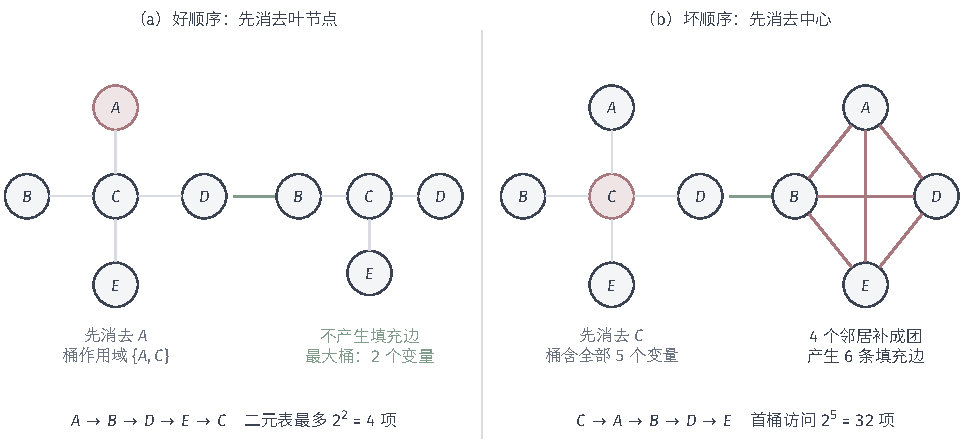
\includegraphics[width=163.153mm]{figures/06-probabilistic-graphical-models/02-inference/tikz/pgm-elimination-order-cost/figure.pdf}
  \caption{五节点二元星形图的两种消元顺序。（a）先消叶节点，每桶至多两个变量且没有填充边；（b）先消中心，首桶枚举$2^5=32$个配置，四个剩余邻居被补成团。红色节点是本步待消变量，红边是新填充边。两边比较稠密表算法的结构代价，最终数值答案保持相同。}
  \label{fig:pgm-elimination-order-cost}
\end{figure*}

在读取函数值前，可以先从作用域预测中间表。构造\term{原始关系图}（primal graph）：把每个当前因子的输入节点两两相连，以图邻接记录同一局部函数中的共同坐标。证据代入后，按剩余实际作用域建图；有向条件表的家庭先形成团，再去掉已固定坐标。这个构造保留因子输入，所得图可以异于原DAG骨架（参考卷一的图论约定）。

当前图中节点$i$的邻居记为$N(i)$。桶积使用$\{i\}\cup N(i)$，消去$i$后输出的作用域为$N(i)$，因此将这些剩余节点两两相连并删除$i$。其中新增的边称为\term{填充边}（fill edge），表示新函数的潜在共同作用域；特定参数仍可能使输出抵消或进一步分解。把该顺序产生的填充边全部保留，得到\term{诱导图}（induced graph）。

消元把内部变量的贡献保存到邻域函数。例如先消$H$，$\sum_h p(h\mid f)\ell_A(h,s)$仍以$f,s$为坐标，填充边$F-S$记录这个输出范围。对每组邻域状态，新表保存桶中子问题的完整汇总，后续直接读取它即可。图的填充说明需要保存哪些坐标，函数值说明每组坐标的数值贡献。

\begin{definition}[诱导宽度与树宽]
  \label{def:pgm-elimination-treewidth}
  对无向交互图$\mathcal{G}$的一条完整消元顺序$\pi$，令$N_t$为消去第$t$个节点之前、已经加入前面填充边后的剩余邻居集合。该顺序的\term{诱导宽度}（induced width）是
  \[
    w(\pi)=\max_t|N_t|.
  \]
  图的\term{树宽}（treewidth）定义为所有完整消元顺序中的最小诱导宽度：
  \[
    \operatorname{tw}(\mathcal{G})=\min_\pi w(\pi).
  \]
  宽度不包含本步被消去的节点，所以最大桶作用域的大小为$w(\pi)+1$。
\end{definition}

树宽给出能够达到的最小剩余邻域上界。森林可逐个消叶；含至少一条边时，其树宽为$1$。$d$节点完全图的首节点总有$d-1$个邻居，故树宽为$d-1$。这两个例子说明，节点数之外还需考虑局部作用域的重叠和可选顺序。

每个离散桶需访问多少状态，由变量基数共同决定。记$r_i=|D_i|$，定义作用域状态数
\[
  D(A)=\prod_{i\in A}r_i,\qquad D(\varnothing)=1.
\]
$D(A)$统计状态组合，集合$A$则指定变量。第$t$桶有$c_t$个因子，合并作用域$U_t=\{i_t\}\cup N_t$；稠密对齐、相乘及汇总使用$O(c_tD(U_t))$次标量操作，输出有$D(N_t)$项。完整保存乘积$\phi_t$需另有$D(U_t)$项工作存储。也可枚举每组$\bm{x}_{N_t}$，在$x_{i_t}$轴累加或取最大，把新增工作表缩至$D(N_t)$项；输入及其它未处理函数仍同时占用空间。

所有状态数至多$r$、输入因子数$m=O(d)$时，宽度$w$的完整顺序给出总运算上界
\begin{equation}
  T=O(d\,r^{w+1}).
  \label{eq:pgm-elimination-discrete-time}
\end{equation}
每个因子只在首个收集它的桶中消耗，每步再产生一个新因子，所以总处理出现次数为$O(m+d)$。去掉$m=O(d)$假设时，上式的$d$相应换为$m+d$。此处按标量运算单位成本计，精确有理数位数的增长另属位复杂度。完整物化桶积的峰值为$O(r^{w+1})$，全部新因子及MPE回溯表可由$O(d\,r^w)$上界，实际同时存活部分可能较小。总空间还包括原输入，因而需分别报告输入、临时乘积及保留输出。

边缘查询只消去$R$，保留$Q$。若显式输出完整查询联合表，最后还需$D(Q)$项。设消元阶段的最大$|N_t|$为$w_R$，无消元步骤时取$w_R=0$，将输出规模也纳入指标：
\[
  \bar w=\max\{w_R,|Q|-1,0\}.
\]
在同一基数条件下，消元与最终表乘积的总时间上界为$O((m+d)r^{\bar w+1})$，输出空间为$D(Q)$项。分析显式输出时，也可预先把$Q$补成团并安排在顺序末尾。普通树宽在全部节点的顺序中优化，此查询则要求保留$Q$，两者的候选顺序集合不同。

两种常用启发式通过当前诱导图选择下一变量。\term{最小度启发式}（min-degree）取剩余邻居最少的节点，控制当前桶的变量数；\term{最小填充启发式}（min-fill）取邻居之间缺边最少的节点，试图减少后续填充。每步补边后重新计算这些指标，才能反映当前函数作用域。局部指标可给出可用顺序，但一般不保证全局最优；最小树宽排序在一般图上是NP难问题，通常先用启发式估计中间表规模，再决定是否执行精确消元\scite{pgm-koller2009}

基数不等时，较少变量也可能组成较大表。例如三个大基数变量的桶可能超过五个二元变量的桶。\term{最小权重启发式}（min-weight）的一种约定据此比较新输出表项数，优先取$\prod_{j\in N(i)}r_j$最小的$i$，等价地比较$\sum_{j\in N(i)}\log r_j$。

若指标针对当前桶的枚举量，则比较$\sum_{j\in\{i\}\cup N(i)}\log r_j$，多计入待消变量的基数。加权填充还可对新增边$(i,j)$使用$r_ir_j$计分，它衡量新连接的成本，与前两种状态数指标不同。这些权重代理计算量，不表示概率。边缘MAP的候选还需满足阶段限制：求和完成前，先在允许求和的节点中选择。

高斯作用域的扩大增加矩阵维度及非零块。一次块消元消去$b$维、保留$a$维，对齐并累加$c_t$个稠密规范因子需$O(c_t(a+b)^2)$。式~\eqref{eq:pgm-elimination-schur}可通过分解与求解实现：Cholesky分解$\bm{J}_{B,B}$需$O(b^3)$，求解$\bm{J}_{B,B}\bm{W}=\bm{J}_{B,A}$需$O(b^2a)$，形成$\bm{J}_{A,B}\bm{W}$需$O(a^2b)$；一次项和常数更新的量级不超过这些主操作。核心更新因此使用
\begin{equation}
  T_{\mathrm{Gauss}}
  =O(b^3+b^2a+ba^2),\qquad
  S_{\mathrm{Gauss}}=O((a+b)^2).
  \label{eq:pgm-elimination-gaussian-cost}
\end{equation}
逐个消标量时$b=1$，对$a$邻居做二次规模更新，总消元典型代价为$O(\sum_t(|N_t|+1)^2)$，另计输入装配。总维度$q$的稠密高斯系统使用$O(q^3)$时间和$O(q^2)$空间，规模按矩阵维数增长。节点代表不同维度块时，成本比较需使用实际$a,b$。

\begin{table}[htbp]
  \centering
  \begin{tabularx}{\linewidth}{@{}lXX@{}}
    \toprule
    比较项 & 离散稠密表格 & 单个高斯规范形式\\
    \midrule
    作用域的表示 & 每种联合状态一项 & 二次项矩阵、一次项向量、常数\\
    合并因子 & 坐标对齐后逐项乘 & 坐标对齐后参数相加\\
    边缘消元 & 对被消去状态求和 & 配方积分与Schur补\\
    主要规模 & 基数乘积$D(U_t)$ & 矩阵块维度$a,b$\\
    填充的后果 & 新表可能指数增大 & 更多非零块与矩阵运算\\
    \bottomrule
  \end{tabularx}
  \caption{离散表与单高斯核的局部计算比较。前者以联合状态索引保存函数，后者以二次矩阵、线性向量和常数保存函数。右列的解析积分适用于单个可归一化高斯核；含离散隐变量后可能增长的混合分量另需计数。}
  \label{tab:pgm-elimination-representation-cost}
\end{table}

边缘MAP把可选顺序限制为两阶段，因而采用查询相关宽度。以$\Pi_{R\prec M}$记全部先排$R$、后排$M$的完整顺序，两组各自内部可任意排列，定义\term{受约束树宽}（constrained treewidth）为
\begin{equation}
  w_{\mathrm{c}}(\mathcal{G};R,M)
  =\min_{\pi\in\Pi_{R\prec M}}w(\pi).
  \label{eq:pgm-elimination-constrained-width}
\end{equation}
某条合法顺序的$w(\pi)$是受约束诱导宽度。候选集合是全部顺序的子集，所以最小值$w_{\mathrm{c}}\geq\operatorname{tw}(\mathcal{G})$。这个指标针对保证任意非负因子正确的两阶段稠密消元，计结构作用域成本；特定函数可交换算子的优势或其它MAP算法的时间下界属于不同分析对象。

执行一条已选合法顺序时，离散时间式~\eqref{eq:pgm-elimination-discrete-time}采用该顺序的实际宽度$w(\pi)$。采用最佳合法顺序才可用$w_{\mathrm{c}}$，得到$O((m+d)r^{w_{\mathrm{c}}+1})$上界；启发式顺序仍可能更宽。受约束树宽因此描述这组顺序可达到的最好结构上界。

以二元星形模型展示普通宽度与受约束宽度的差距。中心$X_0$连接$k$个叶$X_1,\ldots,X_k$，联合积为$p(x_0)\prod_{j=1}^k p(x_j\mid x_0)$。纯求和或MPE先消叶，每步仅一个邻居，普通树宽为$1$。若边缘MAP目标是全部叶，中心需先求和，两阶段算法的第一步为
\begin{equation}
  g(x_1,\ldots,x_k)
  =\sum_{x_0}p(x_0)\prod_{j=1}^{k}p(x_j\mid x_0).
  \label{eq:pgm-elimination-star-map}
\end{equation}
消中心后，$k$个叶成为同一函数的输入并补成团，所以受约束树宽为$k$。物化$g$需要$2^k$项，中心桶要枚举$2^{k+1}$个配置，而初始仅有$O(k)$张常数大小表。图~\ref{fig:pgm-elimination-constrained-star}显示$k=4$时的填充。

\begin{figure}[htbp]
  \centering
  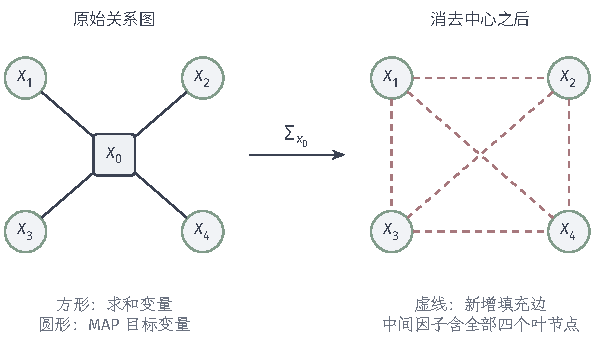
\includegraphics[width=100.651mm]{figures/06-probabilistic-graphical-models/02-inference/tikz/pgm-elimination-constrained-star/figure.pdf}
  \caption{四叶星形模型的边缘MAP消元。左图的目标是四个叶，中心$X_0$先求和；右图用虚线标出新叶间连接，记录四元输出作用域。MPE则允许先消叶，沿此顺序没有这些填充边。}
  \label{fig:pgm-elimination-constrained-star}
\end{figure}

特定参数可让式~\eqref{eq:pgm-elimination-star-map}的输出再次分解，其它算法也可利用这种结构。对仅按作用域操作的通用稠密消元，原图树宽$1$与查询受约束宽度$k$的差别却直接反映中间表增长。这解释了同一图上的边缘MAP为何可能比纯求和和MPE代价更大\scite{pgm-elimination-park2004}

\subsection{实现与适用边界}
\label{sec:pgm-elimination-implementation}

离散表的每一项需要以变量轴和状态编码定位，作用域信息随数值一起保存。相乘前按变量名对齐，或先转置再广播，可以使共享坐标确实表示同一状态。确定性约束产生的零项可用稀疏存储省去；消元后是否继续节省，则取决于新表非零项数。求和合并不同支持、填充扩大坐标范围，都可能令表变稠密，因此先估计峰值作用域，并在运行时记录非零项的实际增长。

高斯模型可用\term{稀疏Cholesky分解}（sparse Cholesky factorization）实现消元：将正定精度矩阵分解为三角因子，保存原非零项及新填充项。排序和符号分析先确定可能填充的位置，数值阶段再计算系数。相同稀疏模式可复用排序与符号结果；复用已有数值分解还要求矩阵值相同。Schur式~\eqref{eq:pgm-elimination-schur}的逆矩阵运算可用三角求解完成，$\log|\bm{J}_{B,B}|$可由分解的对角线计算。

很小的权重连续相乘时，浮点数可能下溢。\term{对数域}（log domain）保存$\log\psi$，将因子乘积改为对数相加，零权重记为$-\infty$。MPE对这些和取最大值，保留同样的回溯索引。边缘查询仍需汇总所有状态，使用对数求和指数式实现这项操作：
\begin{equation}
  \log\sum_i\exp a_i
  =a_{\max}+\log\sum_i\exp(a_i-a_{\max}),
  \qquad a_{\max}=\max_i a_i.
  \label{eq:pgm-elimination-logsumexp}
\end{equation}
当$a_{\max}$有限时，减去它后至少一个指数为$1$，其余不超过$1$，避免直接对大数取指数。全体$a_i=-\infty$表示总权重零，此时直接返回$-\infty$，绕过无定义的无穷相减。若最终查询表处处零，归一化分母也为零，程序返回证据与模型不相容。

中途缩放因子也可控制数值量级。取一个与全部因子坐标无关的$s_t>0$，将$\tau_t$保存为$\widehat{\tau}_t=\tau_t/s_t$；记累计尺度$C_t=\prod_{j=1}^t s_j$，当前不变式相应为
\[
  C_t\prod_{\psi\in\widehat{\mathcal{F}}^{(t)}}\psi
  =\text{原始函数按已执行顺序聚合后的结果}.
\]
累计尺度以$\log C_t=\sum_{j=1}^t\log s_j$保存。条件分布的公共尺度最终抵消，而证据权重及最优绝对得分需恢复它。空作用域的标量因子同样参与这个累计尺度，才能保留原权重。

高斯核的可归一化性需要说明所用空间和测度。完整精度仅半正定、却仍在整个欧氏空间使用规范形式密度时，无二次约束方向的积分会发散。模型若限定在低维仿射子空间，应明确支持及子空间测度，在该空间上积分；伪逆和伪行列式本身不足以表达这些约定。理论正定但数值接近奇异时，检查条件数、变量尺度和分解残差以判断误差放大。对角扰动可以改善数值条件，却同时改动概率模型，应在采用时说明大小及影响。

已知因子分解和明确查询后，可按预计中间作用域判断是否使用精确VE。离散表的高树宽或大受约束宽度可能耗尽内存；单高斯核按矩阵块维度增长，巨大块及填充也会带来高昂代价。相关信息无法全部保存时，第~\ref{chap:pgm-variational}章与第~\ref{chap:pgm-sampling}章分别通过变分和采样完成近似推断。

多次查询还涉及局部计算的复用。同一模型先问$F$再问$S$，从头消元会重复构造部分中间函数。模型与证据允许共享时，可缓存这些汇总，并在后续查询中读取或组合。第~\ref{chap:pgm-junction-tree}章据此组织消息与团树，减少重复工作；作用域本身很大时，其存储成本仍需承担。

\section{本章小结}
\label{sec:pgm-elimination-summary}

故障后验可以从局部因子直接计算：代入报警证据，逐桶相乘并汇总非查询状态，再统一归一化。当前乘积始终等于原函数对已消变量的聚合结果，保证局部替换和完整查询一致。报警例的$p(F=1\mid A=1)\approx0.384111$汇总全部解释，MPE的$(F,H,S)=(0,1,0)$则选择单个联合最优配置，回答不同诊断任务。

查询指定了汇总算子及输出所需信息。边缘概率累加未知状态；MPE取最大值并保存选择，逆序恢复完整配置；边缘MAP先汇总非目标状态，再选目标配置，两算子顺序一般影响答案。目标角色限制可用顺序后，受约束树宽可能大于普通树宽，星形模型也可能生成多叶联合表。

计算代价由顺序产生的作用域和所用函数表示共同决定。离散表按基数乘积保存状态组合，中间规模随诱导宽度指数增长；单高斯规范形式通过矩阵参数相加和Schur补解析更新，成本由块维度及填充决定。选择精确推断时，还需保证归一化合法，并控制浮点尺度与求解误差。中间函数可存放时，VE给出可逐步验证的查询结果；重复查询可进一步共享已有函数，过大的作用域则需要额外结构或明确的近似。

\paragraph{扩展阅读}
Koller与Friedman的教材从因子运算推导变量消除。书中不同顺序的例子可用于比较每桶的输入坐标、输出作用域及状态组合数，进一步理解中间函数为何比原节点总数更直接地决定成本\scite{pgm-koller2009}
